% !TEX program = xelatex
\documentclass[10pt,letterpaper,twocolumn]{article}

% === PAGE ===
\usepackage[top=0.75in,bottom=0.75in,left=0.75in,right=0.75in,footskip=12pt]{geometry}

% === FONTS ===
\usepackage{fontspec}
\usepackage{unicode-math}
\setmainfont{Latin Modern Roman}[
  Extension=.otf,
  UprightFont=lmroman10-regular,
  BoldFont=lmroman10-bold,
  ItalicFont=lmroman10-italic,
  BoldItalicFont=lmroman10-bolditalic,
]
\setsansfont{Latin Modern Sans}[
  Extension=.otf,
  UprightFont=lmsans10-regular,
  BoldFont=lmsans10-bold,
  ItalicFont=lmsans10-oblique,
  BoldItalicFont=lmsans10-boldoblique,
]
\setmonofont{Latin Modern Mono}[
  Extension=.otf,
  UprightFont=lmmono10-regular,
  ItalicFont=lmmono10-italic,
  Scale=0.85,
]
\newfontfamily\acbold{ywft-processing-bold}[
  Path=../../system/public/type/webfonts/,
  Extension=.ttf
]

% === PACKAGES ===
\usepackage{xcolor}
\usepackage{titlesec}
\usepackage{enumitem}
\usepackage{booktabs}
\usepackage{tabularx}
\usepackage{array}
\newcolumntype{Y}{>{\RaggedRight\arraybackslash}X}
\newcolumntype{R}[1]{>{\RaggedRight\arraybackslash}p{#1}}
\usepackage{fancyhdr}
\usepackage{hyperref}
\usepackage{xurl}
\usepackage{graphicx}
\graphicspath{{./}{figures/}}
\usepackage{ragged2e}
\usepackage{microtype}
\usepackage[font=footnotesize]{caption}
\usepackage{natbib}
\usepackage{balance}
\usepackage{tikz}
\usetikzlibrary{arrows.meta,calc,positioning}
\usepackage{../ac-source-bundle}

% === COLORS ===
\definecolor{acpink}{RGB}{180,72,135}
\definecolor{acpurple}{RGB}{120,80,180}
\definecolor{acdark}{RGB}{64,56,74}
\definecolor{acgray}{RGB}{119,119,119}

\hypersetup{
  colorlinks=true,
  linkcolor=acpurple,
  urlcolor=acpurple,
  citecolor=acpurple,
  pdfauthor={@jeffrey},
  pdftitle={Tests It Could Fail: Study Protocols for notepat, AC Native OS and Typing Cadence},
}

% === SECTIONS ===
\titleformat{\section}{\normalfont\bfseries\normalsize\uppercase}{\thesection.}{0.5em}{}
\titlespacing{\section}{0pt}{1.2em}{0.3em}
\titleformat{\subsection}{\normalfont\bfseries\small}{\thesubsection}{0.5em}{}
\titlespacing{\subsection}{0pt}{0.8em}{0.2em}

% === RUNNING MATTER ===
\pagestyle{fancy}
\fancyhf{}
\renewcommand{\headrulewidth}{0pt}
\fancyfoot[C]{\footnotesize\thepage}
\setlist[itemize]{nosep,leftmargin=1.2em,itemsep=0.1em}
\setlist[enumerate]{nosep,leftmargin=1.4em,itemsep=0.1em}
\setlength{\columnsep}{1.8em}
\setlength{\parindent}{1em}
\setlength{\parskip}{0.3em}
\tolerance=800
\emergencystretch=2em
\raggedbottom
\hyphenpenalty=50

\newcommand{\acdot}{{\color{acpink}.}}
\newcommand{\ac}{Aesthetic{\acdot}Computer}
\newcommand{\acos}{AC Native OS}
\newcommand{\np}{\texttt{notepat}}
\newcommand{\code}[1]{\texttt{#1}}
\newcommand{\key}[1]{\texttt{#1}}
\newcommand{\term}[1]{``#1''}

\InputIfFileExists{version}{}{%
  \providecommand{\paperhash}{dev}\providecommand{\paperrev}{?}}

\begin{document}

\twocolumn[{%
\begin{center}
{\acbold\fontsize{24pt}{28pt}\selectfont\color{acdark} Tests It Could Fail}\par
\vspace{0.45em}
{\itshape\fontsize{13.5pt}{16.5pt}\selectfont\color{acpink} Study Protocols for \np{}, \acos{} and Typing Cadence}\par
\vspace{0.6em}
{\small\color{acgray} \href{https://prompt.ac/@jeffrey}{@jeffrey} \,\textperiodcentered\, \ac{} \,\textperiodcentered\, ORCID \href{https://orcid.org/0009-0007-4460-4913}{0009-0007-4460-4913} \,\textperiodcentered\, November 2026}\par
\vspace{0.55em}
{\color{acpink}\rule{\textwidth}{1.2pt}}
\vspace{0.5em}
\end{center}

\begin{quote}
\small\noindent\textbf{Abstract.}
\emph{Don't Forget the Keyboard} placed \np{} and \acos{} in the laptop-performance field and ended on four claims, each paired with the study that would settle it~\citep{scudder2026laptop}. This paper writes those studies down before they run: hypotheses, designs, sample sizes, measures, analyses, and the result that would count against each claim. A fifth study covers the typing-cadence feature Aesel added in the same week. The first study, a wider prior-art search, needed only a search engine. I ran it while writing this paper, and it falsified claim 1: children's Scratch pianos already map the letter \key{c} to the note $C$. The five studies that remain are a 24-hour recall test of the letter-named layout against the DAW's AWSED layout, a cold-boot-to-first-note timing across the fleet, a key-to-sound latency and jitter rig with a tapping task, a listening test of whether a typed melody sounds live, and a test of whether a language model does anything useful with keystroke timing. That last study includes a privacy audit with a decision rule set in advance. Each protocol names its pass line before any data exist.
\end{quote}
\vspace{0.5em}
}]

\section{Why Write the Tests First}

A claim that comes with its own test has to say in advance what result would sink it. \emph{Don't Forget the Keyboard} ended with a table of four claims about \ac{}, each with a nearest prior, a status, and a ``study that settles it''~\citep{scudder2026laptop}. The claims are about systems I built, so I have reasons to read any result kindly. The standard answer to that is pre-registration: fix the hypotheses, the design and the analysis before the data exist, and report any deviation~\citep{nosek2018preregistration,chambers2013registered}. This paper is that registration, written in the open.

The first protocol was cheap enough to run on the day it was written, and it failed the claim it tested (§\ref{sec:s1}). That is the reason to write the others down. The same kind of check that removed the first claim now applies to the rest.

Table~\ref{tab:studies} lists the six studies. Each section below gives the question, the hypothesis, the design, the sample, the measures, the analysis, and a \emph{pass line}: the result that the claim needs. Missing the pass line counts against the claim.

\begin{table*}[t]
\centering
\footnotesize
\renewcommand{\arraystretch}{1.2}
\begin{tabularx}{\textwidth}{@{}R{0.5cm}R{2.6cm}R{3.0cm}R{2.4cm}YR{1.6cm}@{}}
\toprule
\textbf{\#} & \textbf{Claim tested} & \textbf{Design} & \textbf{Sample} & \textbf{Pass line (what the claim needs)} & \textbf{Status} \\
\midrule
1 & No prior maps letters to their own note names. & Multilingual prior-art search: web pianos, patents, code, shareware, Scratch. & 7 queries, 1 fetch. & No letter-named instrument found. & \textbf{Run. Failed.} \\
2 & Letter-named keys are easier to learn. & Two groups, AWSED or \np{} layout; recall at 24\,h. & 40 per group (80\% power for $d \ge 0.64$). & \np{} group recalls more key--note pairs at 24\,h, $p<.05$. & Registered. \\
3 & The laptop boots into one instrument. & Power-on to first audible note, by tapper, across the fleet and four setups. & Every fleet model, 10 boots each. & \acos{} faster than every comparison, on every machine. & Registered. \\
4 & Latency is inside the intimacy budget. & Tapper and two-channel rig; then human tapping to a metronome. & 1000 strikes per setup; 24 tappers. & Mean ${\le}\,10$\,ms and jitter ${\le}\,1$\,ms on HDA; no added tapping variance. & Registered. \\
5 & A typed melody sounds live. & Listening test after Bown et al.; audio-only and with video. & 120 listeners online. & Typed excerpts rated no less live than tweaked ones, audio-only. & Registered. \\
6 & Keystroke timing helps a model reply. & Same messages with and without cadence; blind pairwise raters; plus a re-identification audit. & 60 messages, 2 models, 5 raters; 20 typists. & Cadence replies preferred, with no timing remarks; audit decides what is sent. & Registered. \\
\bottomrule
\end{tabularx}
\caption{The six studies. Studies 1--5 test the four claims of \citet{scudder2026laptop}, with claim 1 split into priority (Study 1) and learnability (Study 2); Study 6 tests Aesel's cadence feature (§\ref{sec:s6}). The pass line is fixed here, before any data, and missing it counts against the claim.}
\label{tab:studies}
\end{table*}

\section{Study 1: Is the Mapping New?}
\label{sec:s1}

\paragraph{Question.} Has any instrument before \np{} made the letter on a key play the note with that name, so that \key{c} plays $C$?

\paragraph{Design.} The first paper's search found none in two targeted queries and named where it had not looked: patents, Japanese and German web pianos, and pre-web shareware~\citep{scudder2026laptop}. This pass searched those, plus code repositories and Scratch. Each query ran through \ac{}'s Exa-backed search service, and each hit was opened at its primary page. The kill line was set before searching: \emph{one} instrument that plays at least five of the seven natural notes from their own letters breaks the claim.

\paragraph{Result.} The claim failed. Japanese and German web pianos were all positional: the AWSED row, the 61-key number-row layout, or the bottom row~\citep{webmusic_ja,toolsforanyone_de}. The patents placed notes by how often they are played~\citep{patent6444888}. The DOS archive and the code search turned up only positional and ASCII maps. Scratch broke the claim twice. Harvard's ScratchEd site hosts a classroom tutorial in which children make one letter sprite per note: ``press the C key and the note will play''~\citep{sienna_scratchpiano}. A 2018 project, \emph{Keyboard on Scratch}, plays a whole chromatic octave this way, ``press the note letters to play the notes,'' with sharps on \key{h}--\key{l}~\citep{persam2018scratch}.

\paragraph{What survives.} A narrower fact, not a priority claim. \np{} carries the letter-named octave into a second octave on \key{h}--\key{n} and uses it as a performance instrument and the shell of an operating system. The Scratch result also bears on Study 2. When a child is asked to build a piano out of letters, this is the mapping the child builds. That counts for the learnability hypothesis, but it does not prove it.

\begin{figure*}[t]
\centering
% Measurement rig for Studies 3 and 4: a tapper strikes a laptop key, a piezo
% on the keycap marks the strike, and the laptop's audio output is recorded on
% a second channel of the same interface, so both onsets share one clock.
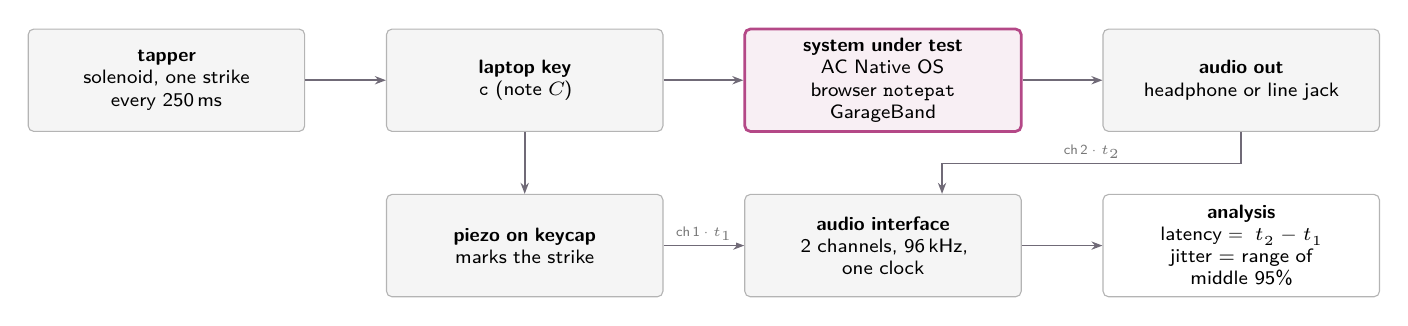
\begin{tikzpicture}[
  every node/.style={font=\sffamily},
  box/.style={draw=acgray!55, fill=acgray!7, rounded corners=2pt, align=center,
    minimum height=1.3cm, text width=3.3cm, font=\scriptsize\sffamily, inner sep=3pt},
  dut/.style={box, draw=acpink, line width=1.0pt, fill=acpink!9},
  sink/.style={box, fill=white},
  arr/.style={-{Stealth[length=4pt]}, draw=acdark!75, line width=0.6pt},
  lab/.style={font=\tiny\sffamily, text=acgray, fill=white, inner sep=1.5pt}
]
  % top row: the action path
  \node[box] (tap) at (0,0) {\textbf{tapper}\\solenoid, one strike\\every 250\,ms};
  \node[box] (key) at (4.55,0) {\textbf{laptop key}\\\key{c} (note $C$)};
  \node[dut] (sys) at (9.1,0) {\textbf{system under test}\\\acos{}\\browser \np{}\\GarageBand};
  \node[box] (jack) at (13.65,0) {\textbf{audio out}\\headphone or line jack};
  % bottom row: the measuring path
  \node[box] (piezo) at (4.55,-2.1) {\textbf{piezo on keycap}\\marks the strike};
  \node[box] (iface) at (9.1,-2.1) {\textbf{audio interface}\\2 channels, 96\,kHz,\\one clock};
  \node[sink] (ana) at (13.65,-2.1) {\textbf{analysis}\\latency $= t_2 - t_1$\\jitter = range of\\middle 95\%};

  \draw[arr] (tap) -- (key);
  \draw[arr] (key) -- (sys);
  \draw[arr] (sys) -- (jack);
  \draw[arr] (key) -- (piezo);
  \draw[arr] (piezo) -- node[lab, above] {ch\,1 $\cdot$ $t_1$} (iface);
  \draw[arr] (jack.south) -- ++(0,-0.4) -| node[lab, pos=0.25, above] {ch\,2 $\cdot$ $t_2$} ($(iface.north)+(0.75,0)$);
  \draw[arr] (iface) -- (ana);
\end{tikzpicture}

\caption{The rig for Studies 3 and 4. The pink box is the system under test. A solenoid strikes the key every 250\,ms, as in McPherson et al.'s method~\citep{mcpherson2016latency}. A piezo on the keycap ($t_1$) and the laptop's audio output ($t_2$) go to two channels of one interface, so both onsets share one clock. Latency is $t_2 - t_1$. Jitter is the spread of the middle 95\% of 1000 strikes.}
\label{fig:rig}
\end{figure*}

\section{Study 2: Learning the Letter-Named Keys}
\label{sec:s2}

\paragraph{Question.} Do novices learn and keep key--note pairs faster when the letter on the key is the note's name?

\paragraph{Hypothesis.} H2: 24 hours after a short lesson, people who learned \np{}'s layout recall more key--note pairs than people who learned the AWSED layout, the DAW convention in which \key{a} plays $C$ and \key{s} plays $D$~\citep{scudder2026keymaps}.

\paragraph{Participants.} Adults who type but do not play a keyboard instrument. Screening excludes anyone who reports more than one year of piano or keyboard lessons, and anyone who has used \np{} or a DAW's musical typing. Forty per group gives 80\% power to detect a standardized difference of $d = 0.64$ at $\alpha = .05$, two-sided~\citep{cohen1988power}. Jordà's ``low entry fee'' predicts a large effect, and this design will not detect a small one~\citep{jorda2004efficiency}.

\paragraph{Procedure.} Participants are randomly assigned to one of two layouts, both run in the browser build of \np{} with key labels hidden. A 15-minute lesson teaches three melodies, written as note names (\emph{E D C D E E E}), as children's songbooks print them. Practice ends when each melody is played once without error, or at 15 minutes. At 24 hours, an online test shows 14 note names in random order (both octaves' naturals) and asks for the key. It then shows one unseen melody as note names and asks for it to be played.

\paragraph{Measures.} Primary: the number of correct key--note pairs at 24\,h, out of 14. Secondary: lesson time to the first error-free melody; transfer accuracy on the unseen melody; and, as a cost check, the number of piano-position errors. AWSED keeps the piano's white--black geometry and \np{} does not, so the AWSED group might transfer better to a real piano.

\paragraph{Analysis and pass line.} A two-sample comparison of the primary measure (Welch's $t$; Mann--Whitney if the distribution is badly skewed). Per-item correctness goes into a mixed-effects logistic model with random intercepts for participant and item. H2 passes if the \np{} group recalls more pairs, $p < .05$. A null result with a confidence interval that excludes $d = 0.64$ counts against the learnability argument made in \emph{Keymaps}.

\section{Study 3: Boot to First Note}
\label{sec:s3}

\paragraph{Question.} How long does it take to get from a powered-off laptop to an audible note, and how many human actions does it take?

\paragraph{Hypothesis.} H3: on every laptop in the fleet, \acos{} reaches the first note sooner, and in fewer actions, than every comparison setup on the same machine.

\paragraph{Setups.} (a) \acos{} from USB. (b) The machine's installed operating system, browser, and \np{} at its URL. (c) GarageBand's Musical Typing, on Macs only. (d) MOD's live USB, measured to its first audible output where the laptop's onboard audio is supported. Each setup is timed on the same machine, so the hardware cancels out.

\paragraph{Procedure.} The tapper from Study 4 (Figure~\ref{fig:rig}) strikes \key{c} every 250\,ms from the moment the power button is pressed. A contact microphone marks the power press; the headphone output is recorded. Boot-to-first-note is the time from the press to the first audio onset above $-40$\,dBFS. Steps that need a person (log in, open a browser, type a URL, choose a patch) are done by one operator, as fast as possible, following a written script, and counted. Ten cold boots per setup per machine, with full power-off between boots.

\paragraph{Measures and pass line.} Median and range of boot-to-first-note, and the count of human actions. \acos{}'s 7.3\,s boot to PID 1 is a lower bound, not the measure~\citep{scudder2026os}. H3 passes if \acos{}'s median is lower than every comparison's on every machine. A machine where it is not is reported by model, along with the reason.

\section{Study 4: Latency and Jitter}
\label{sec:s4}


\paragraph{Question.} Is the key-to-sound path inside Wessel and Wright's budget of 10\,ms latency and 1\,ms variation, and does whatever jitter it has show up in a player's timing~\citep{wessel2002problems}?

\paragraph{Why jitter.} \emph{Where the Microseconds Go} reports a mean of 3--4\,ms on HDA codecs and 12--22\,ms on SOF, with no jitter figure~\citep{scudder2026latency}. The mean is the wrong number to stop at. Jack, Stockman and McPherson gave percussionists an instrument at 10\,ms, at 20\,ms, and at 10\,ms with $\pm3$\,ms jitter. The jittered condition was rated about as badly as 20\,ms, while steady 10\,ms was rated like zero~\citep{jack2016latency}. McPherson, Jack and Moro measured common maker setups and found jitter above 1\,ms in every configuration except Bela~\citep{mcpherson2016latency}.

\paragraph{Part A: the rig.} 1000 strikes per setup, 250\,ms apart (Figure~\ref{fig:rig}). Setups: \acos{} on an HDA laptop and on an SOF laptop; the browser build of \np{} on the same laptops' installed systems; and GarageBand's Musical Typing on a Mac. Jitter follows McPherson et al.: discard the top and bottom 2.5\% of trials, then take the range of the rest~\citep{mcpherson2016latency}. The rig's own error is measured first, with the piezo signal fed to both channels.

\paragraph{Part B: people.} 24 participants tap along with a metronome on \key{f} at intervals of 500, 333 and 250\,ms, on \acos{} and on the slowest setup from Part A, in counterbalanced order. The measure is the standard deviation of asynchrony, the stability index of the tapping literature~\citep{repp2005sms}. Tap times come from the piezo, not from the software, so the system's own jitter cannot hide in the measurement.

\paragraph{Pass line.} H4a: on HDA, mean latency ${\le}\,10$\,ms and jitter ${\le}\,1$\,ms. H4b: asynchrony SD on \acos{} is no larger than on the slow setup; this is a non-inferiority test with a margin of 2\,ms. SOF laptops are expected to fail H4a and are reported as such.

\section{Study 5: Does a Typed Melody Sound Live?}
\label{sec:s5}

\paragraph{Question.} The liveness critique says a laptop audience cannot see the cause of the sound~\citep{cascone2003grain,collins2003generative}. Bown, Bell and Parkinson found that listeners, from audio alone, hear \emph{triggering} as more live than tweaking~\citep{bown2014liveness}. Is a typed melody, which is pure triggering, heard as live?

\paragraph{Design.} Following Bown et al.'s approach, listeners rate short excerpts, without knowing how they were made, on how much of what they hear the performer is doing at that moment. There are three sources: (i) a melody typed live on \np{}; (ii) the same notes played back from a sequence; (iii) a generative patch whose parameters the performer tweaks live. Modality is between subjects: one group hears audio only, the other sees video of the hands and the screen, with the letters visible. 120 listeners online, 60 per group, each rating 18 excerpts in random order.

\paragraph{The trap in the design.} In audio only, (i) and (ii) are the same audio. Listeners cannot tell them apart, so any difference between them is noise. That makes (ii) a manipulation check. The claim lives in two other comparisons: typed against tweaked in audio only, and the gain from adding video.

\paragraph{Analysis and pass line.} An ordinal mixed model with random effects for listener and excerpt. H5a: in audio only, typed excerpts are rated no less live than tweaked ones; this is a non-inferiority test with a margin of half a scale point. H5b: video raises ratings for typed excerpts more than for tweaked ones (the interaction). If typed excerpts are rated \emph{less} live than tweaked ones in audio only, the argument in the first paper fails.

\section{Study 6: Does a Model Listen to Typing?}
\label{sec:s6}

\paragraph{Question.} Aesel now attaches each message's keystroke timing to the prompt it sends to the model. The timing includes interval quantiles, pauses of 2\,s or more, bursts, erases and pasted characters, and never which keys~\citep{scudder2026aesel}. Does a model reply better with that context, and does sending it leak who is typing?

\paragraph{Part A: usefulness.} Sixty real messages from the author's own Aesel sessions, each with its recorded cadence, are sent to two models twice: once with the cadence block and once without. Five raters who do not know which reply is which see the message and two replies in random order, and choose the one that better fits what the person needed. A second set holds the text fixed and swaps in a cadence from a different message: hurried for hesitant, typed for pasted. That set tests whether the replies move with the timing and whether the movement is appropriate. Raters also flag any reply that \emph{mentions} the timing.

\paragraph{Pass line A.} H6a: replies with cadence are preferred in more than half of the pairs (binomial test across raters, with message as a random effect), and fewer than 5\% of replies remark on the timing. If replies with cadence are not preferred, the feature should be turned off by default.

\paragraph{Part B: the privacy audit.} Keystroke timing identifies typists; Killourhy and Maxion's benchmark exists for that purpose~\citep{killourhy2009comparing}. Twenty consenting typists each produce 30 cadence summaries in ordinary use. A scaled-Manhattan detector, one of the strongest in that benchmark, is trained on each typist's first 15 summaries and tested on the rest~\citep{killourhy2009comparing}. The equal-error rate is reported twice: once with the raw interval list (\code{gapsMs}) and once with only the summary statistics.

\paragraph{Decision rule.} Set now: if the raw interval list gives an equal-error rate below 15\%, Aesel stops sending \code{gapsMs} by default and keeps only quantiles, pauses and counts. Then the audit runs again. The rule is set in advance so that the result decides the default, not the author's preference.

\section{Shared Procedures}

\paragraph{Consent and data.} Studies 2, 4B, 5 and 6 involve people. Each participant gets a plain-language description of what is recorded and why. In Study 5 the video shows hands and screens only, never faces. Study 6 records timing and never key identities, and the audit's summaries are deleted after analysis. Where an institution is involved, its ethics review comes first.

\paragraph{Deviations.} Anything that changes after this paper is fixed (a sample size, a setup, an exclusion) will be listed in the results paper with its reason. A study that cannot run, such as MOD on unsupported hardware, is reported as not run, not dropped.

\paragraph{Materials.} The tapper firmware, the onset-detection script, the lesson melodies, the listening excerpts and the analysis code will go into this paper's source bundle and the \texttt{laptop-platter} before data collection starts.

\section{Limitations}

These are small studies by one person, and most of their participants will come from the communities around \ac{}. Study 2 can detect only a large effect. Study 3 measures the fleet I own, which is surplus hardware, not a sample of laptops. In Study 5, an excerpt chosen by the author is an excerpt the author likes. The excerpts will be cut by a fixed rule (the first 20\,s after the first note) to limit that. Study 6's messages are the author's own, so its raters judge replies to one person's typing.

Study 1 is the reminder. A negative search is bounded by where it looked, and the place that broke it, children's coding projects, was not on the first list of places to look.

\section{Conclusion}

The first paper's claims now each have a test written down, and one of them has already failed. The letter-named key is not \ac{}'s idea; it is what a child builds when asked to make a piano from letters. That leaves a narrower set of claims to defend: a second octave and an instrument built on the mapping, a laptop that boots into it, a latency budget, a liveness argument, and a guess that the gaps between keys say something a model can use. Each of these now has a pass line set before its data exist.

\bibliographystyle{plainnat}
\balance
\setlength{\bibsep}{0pt}
{\footnotesize\bibliography{references}}

\vspace{0.8em}
\begin{center}
\footnotesize\sffamily\color{acgray}
Revision \paperrev\;\textperiodcentered\;\texttt{\paperhash}\;\textperiodcentered\;
\href{https://papers.aesthetic.computer/laptop-protocols-26-arxiv.pdf}{papers.aesthetic.computer/laptop-protocols-26-arxiv}
\end{center}

\end{document}
